\chapter{Niet-Programmeerbare Processoren}
\chapterquote{We accepteren nu het feit dat leren een levenslang proces is om op de hoogte te blijven van veranderingen. En de meest urgente taak is mensen te leren hoe te leren.}{Peter F. Drucker, Amerikaans management consultant en auteur (1909-)}
\begin{chapterintro}
In de twee vorige hoofdstukken hebben we componenten gebouwd met een beperkte functionaliteit. De combinatorische schakelingen laten ons toe om schakelingen te ontwerpen die een rekenkundige operatie uitvoeren, maar we hebben geen geheugen beschikbaar om tussenresultaten in op te slaan. Het hoofdstuk over sequenti\"ele schakelingen maakt het mogelijk om schakelingen te ontwerpen met een geheugen. De meeste problemen hebben echter zeer grote toestandsruimtes (een 32-bit getal heeft meer dan vier miljard toestanden). Daarom volstaan de methodes uit dit hoofdstuk niet om een component te ontwikkelen die iets functioneel doet. Daarvoor zullen we methodes op een hoger niveau introduceren, dat van een niet-programmeerbare processor. Een niet programmeerbare processor voert een algoritme uit die op voorhand gekend is. Hierdoor kunnen we optimaal gebruik maken van de hardware en zoveel mogelijk instructies tegelijk uitvoeren. Het nadeel is dat eenmaal de processor geproduceerd is, we geen andere problemen met het component kunnen uitvoeren.
\end{chapterintro}
\minitoc[n]
\section{De Niet-Programmeerbare Processor}
Alvorens we de bouw van zo'n processor verder uitwerken, dienen we eerst enkele concepten te formaliseren. Allereerst ontleden we in deze sectie uit welke delen zo'n processor is opgebouwd. Vervolgens zullen we in sectie \ref{s:descriptionFSMD} een methode ontwikkelen om een algoritme formeel weer te geven. Deze beschrijving zal toelaten het algoritme later om te zetten naar een processor. In sectie \ref{s:memoryFSMD} ten slotte zullen we extra geheugencomponenten introduceren die we nodig zullen hebben bij de bouw van een processor.
\subsection{Algemene Structuur}
Een \termen{Niet-programmeerbare processor}, ofwel \termen{Finite State Machine with Data path (FSMD)} bestaat grofweg uit twee delen:
\begin{itemize}
 \item Een \termen{datapad}: een component die bewerkingen (rekenkundig, aritmetisch,...) uitvoert en de resultaten opslaat in tijdelijk geheugen.
 \item Een \termen{controller}: een component die het datapad aanstuurt. Het zegt welke actie op welk moment moet ondernomen worden.
\end{itemize}
In dit hoofdstuk is de controller niet programmeerbaar. Dat wil zeggen dat de controller telkens hetzelfde programma uitvoert. Dit betekent echter niet dat er een vaste cyclus in de controller zit. De controller kan afhankelijk van de waarden die in de geheugens van het datapad zitten, of van ingangen van de processor beslissen om andere acties te ondernemen. Een controller is dus een sequenti\"ele schakeling ofwel finite state machine. De synthese van een finite state machine werd in het hoofdstuk \ref{ch:SeqComp} reeds besproken. Uiteraard zullen we de karakteristieken die eigen zijn aan controllers in dit hoofdstuk bespreken.
\paragraph{}
Het spreekt voor zich dat de controller en het datapad continu data met elkaar uitwisselen. Enerzijds geeft de controller instructies aan het datapad. De groep signalen waarmee een controller een datapad aanstuurt noemen we het ``\termen{instructiewoord}'' ofwel ``\termen{controle-signalen}''. Anderzijds zullen de instructies vaak afhangen van de toestand van variabelen opgeslagen in het datapad. De verzameling van signalen die het datapad over zijn variabelen doorstuurt naar de controller noemen we ``\termen{statussignalen}''.
\paragraph{}
Een processor voert operaties uit op data. Deze data moet op de een of andere manier ingelezen worden in de processor. De verzameling ingangen waarmee we data vanuit de omgeving in het datapad injecteren noemen we de ``\termen{data-ingangen}''. Verder zullen we vaak ook informatie aan de controller moeten meedelen: we denken bijvoorbeeld aan een signaal die actief wordt wanneer alle data ingelezen is, en het algoritme kan uitgevoerd worden. Deze signalen noemen we ``\termen{controle-ingangen}''. Daarnaast willen we ook de resultaten kunnen uitlezen. Hiervoor voorzien we een reeks signalen vanuit het datapad, deze signalen noemen we ``\termen{data-uitgangen}''. Tot slot zijn we soms ook ge\"interesseerd in de toestand van het algoritme. We zullen bijvoorbeeld enkel data uitlezen indien het algoritme afgelopen is. De controller kan informatie over het algoritme naar buiten brengen via ``\termen{controle-uitgangen}''. De verschillende informatiestromen tussen het datapad en de controller en de processor en zijn omgeving beschrijven we op figuur \ref{fig:processorInformationStreams}.
\begin{figure}[hbt]
\centering
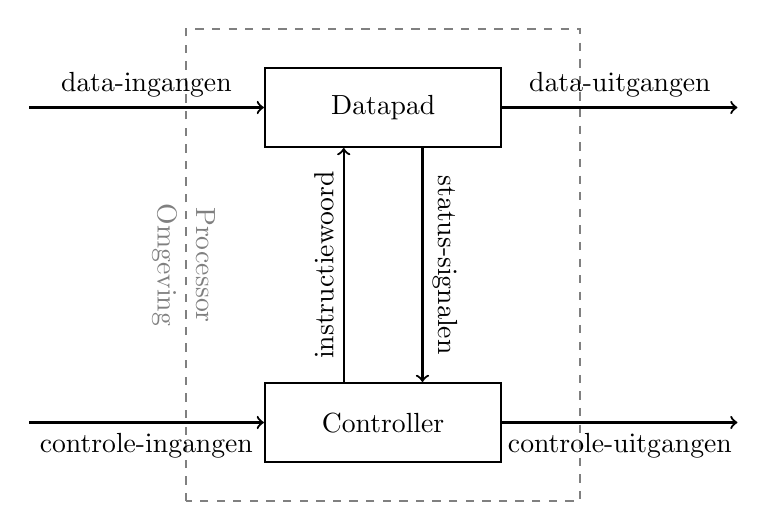
\begin{tikzpicture}
\draw[gray,dashed,thick] (-2.5,-3) rectangle (2.5,3);
\draw (-2.5,0) node[rotate=-90,gray,anchor=south]{Processor};
\draw (-2.5,0) node[rotate=-90,gray,anchor=north]{Omgeving};
\node[rectangle,thick,draw=black,minimum width=3 cm,minimum height=1 cm] (D) at (0,2) {Datapad};
\node[rectangle,thick,draw=black,minimum width=3 cm,minimum height=1 cm] (C) at (0,-2) {Controller};
\draw[->,thick] (D.south -| 0.5,0) to node[midway,sloped,above]{status-signalen} (C.north -| 0.5,0);
\draw[->,thick] (C.north -| -0.5,0) to node[midway,sloped,above]{instructiewoord} (D.south -| -0.5,0);
\draw[<-,thick] (C.west) to node[below,midway]{controle-ingangen} (-4.5,-2);
\draw[->,thick] (C.east) to node[below,midway]{controle-uitgangen} (4.5,-2);
\draw[<-,thick] (D.west) to node[above,midway]{data-ingangen} (-4.5,2);
\draw[->,thick] (D.east) to node[above,midway]{data-uitgangen} (4.5,2);
\end{tikzpicture}
\caption{Opbouw van een processor.}
\label{fig:processorInformationStreams}
\end{figure}
\paragraph{}
Door de controle-ingangen wordt de definitie van ``niet-programmeerbaar'' natuurlijk vaag. We zouden immers het toestandswoord van de controller in grote mate laten afhangen van de invoer die de controle-ingangen. Hierdoor kunnen we de processor toch programmeren. Het onderscheid is dan ook eerder een common-sense.
\subsection{Het Datapad}
\section{Formeel Beschrijven van een Algoritme}
\label{s:descriptionFSMD}
\section{Geheugencomponenten}
\label{s:memoryFSMD}
\section{Synthese van een Niet-Programmeerbare Processor}
\label{s:syntheseFSMD}
\section{Tijdsgedrag}
\label{s:timeFSMD}